\documentclass[a4paper,10pt]{article} 
\usepackage[utf8]{inputenc}
\usepackage[a4paper]{geometry}
\usepackage[magyar]{babel}
\usepackage{t1enc}
\usepackage{amsmath}
\usepackage{amssymb}
\usepackage{pgf,tikz,longtable}
\usetikzlibrary{arrows}
\frenchspacing 
\pagestyle{empty}
\newcommand{\ki}[2]{\hfill {\it #1 (#2)}\medskip}
\newcommand{\vonal}{\hbox to \hsize{\hskip2truecm\hrulefill\hskip2truecm}}
\newcommand{\degre}{\ensuremath{^\circ}}
\newcommand{\tg}{\mathop{\mathrm{tg}}\nolimits}
\newcommand{\ctg}{\mathop{\mathrm{ctg}}\nolimits}
\newcommand{\arc}{\mathop{\mathrm{arc}}\nolimits}
\begin{document}
\begin{center} \Large {\em 23. Nemzetközi Magyar Matematika Verseny} \end{center}
\begin{center} \large{\em Csíkszereda, 2014. március 12-16.} \end{center}
\smallskip
\begin{center} \large{\bf 10. osztály} \end{center}
\bigskip 

{\bf 1. feladat: }  Oldd meg a prímszámok halmazán a $$
3x^{2}-y^{2}=22y-12x$$ egyenletet!


\ki{Olosz Ferenc}{Szatmárnémeti}\medskip

{\bf 1. megoldás: }  Az egyenletet rendezzük az ismeretlenek szerint
és mind\-két oldalt szor\-zat\-tá alakítjuk:%
\[
3x(x+4)=y(y+22).%
\]
A bal oldal osztható $3$-mal. Ha $y=3$, akkor az $x^{2}+4x-25=0$
egyenlethez jutunk és ennek nincs egész megoldása.  Ha
$x=y$, akkor $3x+12=x+22$, ahonnan $x=y=5$ prímszám,
tehát megoldás. Az $x$ és $y$ prímszám volta
miatt csak $3x\mid(y+22)$ és $y\mid(x+4)$ lehetséges. Ekkor
$y\leq x+4\leq\frac{y+22}{3}+4$ és kapjuk, hogy $y\leq17$.
Másrészt $3\mid(y+22)$, így csak az
$$y\in\left\{ 2,5,11,17\right\}  $$ értékek lehetségesek.
Ezeket kipróbálva, az $\left( 5,5\right)$ és $\left(
13,17\right)$ meg\-oldá\-sok\-hoz jutunk.




\medskip

{\bf 2. megoldás: }  $x = y$  esetén az egyenlet egyetlen megoldása $x = y = 5.$
Ha  $x\neq y,$  akkor az egyenletet átírva, a $p\in \mathbb{N}$
változó beve\-ze\-té\-sé\-vel írhatjuk, hogy
\[\frac{{3(x + 4)}}{y} = \frac{{y + 22}}{x} = p,\] ahonnan  \[x =
\frac{{22p + 12}}{{{p^2} - 3}}  \mbox{ és } y = \frac{{12p +
66}}{{{p^2} - 3}}.\] Itt $p = 3$  esetben megkapjuk az  $x = 13, y =
17$ megfe\-le\-lő meg\-ol\-dást, a többi  $p$  értékekre  $1$-
től $16$-ig nem kapunk jó megoldást. Ha $p\geq 17,$ akkor  már
$y<1,$ ezért nincs több megoldás.

\medskip

\textit{Megjegyzés}: Az előbb kapott kifejezések $p\in \mathbb{Q}$ esetén az
egyenlet végtelen sok racionális megoldását adják, közöttük
végtelen sok egész megoldás is van.

\medskip

\vonal


{\bf 2. feladat: }  Négy Tudós Matematikus egy egyenlő szárú trapéz alakú birtokon
él, házaik a trapéz csúcsaira épültek. A trapéz hosszabb alapjának
hossza $a$, az alapon fekvő szögek nagysága $50^\circ $, az átlók
által bezárt szög pedig $76^\circ$. A Tudósok szeretik a szabályos
dolgokat, így elhatározták, hogy olyan kutat építenek, amely
mindannyiuk házától ugyanolyan távolságra helyezkedik el. Milyen
távolságra kell építeniük házaiktól a kutat? Vajon a kút a
birtokukon lesz-e?


\ki{dr. Péics Hajnalka}{Szabadka}\medskip

{\bf Megoldás: }   Ahhoz, hogy minden háztól ugyanolyan távolságra le\-gyen,
a kutat a trapéz köré írt kör középpontjába kell elhelyezni.

Jelölje $A$, $B$, $C$, $D$ a trapéz csúcspontjait, $E$ a trapéz
átlóinak metszéspontját, $O$ pedig a trapéz köré írható körének
kö\-zép\-pont\-ját. Legyen $AB$ a trapéz hosszabb alapja. Tudjuk,
hogy ${CEB}\sphericalangle$ vagy ${AEB}\sphericalangle$ $76^\circ$-os. Az
${AEB}\sphericalangle$ azonban nem lehet $76^\circ $, mert ellenkező
esetben az ${EAB}\sphericalangle$ és ${EBA}\sphericalangle$ nagysága $52^\circ $
lenne (az $ABE\Delta $ egyenlő szárú), ami nem lehetséges, mert
ezek a szögek a trapéz alapon fekvő szögeinél, a
${DAB}\sphericalangle$-nél és ${CBA}\sphericalangle$-nél kisebbek, tehát $50^\circ
$-nál kisebbek kell legyenek. Eszerint ${CEB}\sphericalangle = 76^\circ $,
ahonnan ${AEB}\sphericalangle= 180^\circ - 76^\circ  = 104^\circ $,
valamint ${ABE}\sphericalangle = \frac{{180^\circ - 104^\circ }}{2} =
38^\circ $. Továbbá az $AB$ húr kerületi szöge $${ADB}\sphericalangle =
180^\circ  - ({DAB}\sphericalangle + {ABE}\sphericalangle) = 92^\circ ,$$ ami
szerint az $AB$ húr középponti szöge $${AOB}\sphericalangle =
2{ADB}\sphericalangle = 184^\circ
> 180^\circ .$$ Ebből az következik, hogy a trapéz köré írt
kör $O$ középpontja a trapéz belső tartományán kívül esik. Ez azt
jelenti, hogy a kutat nem lehet úgy megépíteni a Négy Tudós
mate\-ma\-ti\-kus birtokára, hogy mindannyiuktól ugyanolyan
távolságra legyen. Mivel ${BAO}\sphericalangle  = 2^\circ $ és $\cos
2^\circ  = \frac{{\frac{a}{2}}}{r}$, ahol $r$ a trapéz köré
írt kör sugara, következik, hogy $r = \frac{a}{{2\cos 2^\circ
}}$. Ez azt jelenti, hogy a kút minden háztól $r = \frac{a}{{2\cos
2^\circ }}$ távolságra kell legyen.

\medskip

\textit{Megjegyzés}: Az  $ABCD$  trapéz köré írható kör megegyezik az  $ABD$
háromszög köré írható körrel. A szinusz tétel alapján
\[\frac{{AB}}{{\sin {ADB}\sphericalangle}} = 2r,\] ami az
 $\frac{a}{{\sin {{92}^ \circ }}} = 2r$ egyenlőséghez vezet. Innen következik, hogy
 \[r = \frac{a}{{2\cos {2^ \circ }}}.\]

\medskip 

\vonal

{\bf 3. feladat: } Oldd meg a pozitív valós számok halmazán a $$
\displaystyle 2^{4x+1}+2^{\frac{1}{2x^{2}}}=12 $$
 egyenletet!

\ki{Koczinger Éva és Kovács Béla}{Szatmárnémeti}\medskip


{\bf 1. megoldás: } Az egyenlet bal oldalát úgy alakítjuk, hogy
al\-kal\-maz\-has\-suk három po\-zi\-tív szám számtani és mértani
középarányo\-sa közötti egyenlőtlenséget.
\[{2^{4x + 1}} + {2^{\frac{1}{{2{x^2}}}}} = 2 \cdot {2^{4x}} +
{2^{\frac{1}{{2{x^2}}}}} = {2^{4x}} + {2^{4x}} + {2^{\frac{1}{{2{x^2}}}}}\geq\]
   \[\geq 3 \cdot \sqrt[3]{{{2^{4x + 4x + \frac{1}{{2{x^2}}}}}}} = 3
   \cdot {2^{\frac{{4x + 4x + \frac{1}{{2{x^2}}}}}{3}}}\geq\]
     \[\geq 3 \cdot {2^{\sqrt[3]{{4x \cdot 4x \cdot \frac{1}{{2{x^2}}}}}}} = 3
      \cdot {2^2} = 12\]  és ez  pontosan az egyenlet jobb oldala.
Egyenlőség pontosan akkor teljesül, ha a kö\-zép\-a\-rá\-nyosok
közötti egyenlőtlenséget egyenlő számokra alkalmaztuk.
Ezért ${2^{4x}} = {2^{\frac{1}{{2{x^2}}}}}$, és így
    \[4x = \frac{1}{{2{x^2}}} \Leftrightarrow x = \frac{1}{2}.\]
Ez valóban megoldása az adott egyenletnek.

\medskip

{\bf 2. megoldás: }  Átalakítjuk az egyenletet:
$${2^{4x}} + {2^{4x}} + {2^{\frac{1}{{2{x^2}}}}} + {2^2} = {2^4},$$
majd a bal oldalon kétszer alkalmazzuk a számtani és mértani
közepek közti egyenlőtlenséget:
$$16 = {2^{4x}} + {2^{4x}} +
{2^{\frac{1}{{2{x^2}}}}} + {2^2} \geqslant 2\sqrt {{2^{8x}}}  +
2\sqrt {{2^{\frac{1}{{2{x^2}}} + 2}}}  \geqslant$$ $$ \geqslant
4\sqrt[4]{{{2^{8x + \frac{1}{{2{x^2}}} + 2}}}} = {2^{\frac{{^{8x +
\frac{1}{{2{x^2}}} + 2}}}{4} + 2}} = {2^{^{\frac{8x +
\frac{1}{{2{x^2}}} + 10}{4}}}}.$$ Ez ekvivalens a $$8x +
\frac{1}{{2{x^2}}} + 10 \leqslant 16$$ egyenlőtlenséggel és
ebből $$\frac{{16{x^3} - 12{x^2} + 1}}{{2{x^2}}} \leqslant 0.$$
Tényezőkre bontva: $\frac{{{{\left( {2x - 1} \right)}^2}\left(
{4x + 1} \right)}}{{2{x^2}}} \leqslant 0$. Ez csak akkor lehetséges,
ha $x = \frac{1}{2}.$ Ezt az értéket visszahelyettesítve az
eredeti egyenletbe, igaz egyenlőséghez jutunk, tehát $x =
\frac{1}{2}$ az egyetlen pozitív megoldása az adott egyenletnek.

\medskip

\textit{1. megjegyzés}: A számolás közben a következő felbontást
vé\-gez\-tük:
  $$16{x^3} - 12{x^2} + 1 = 16{x^3} - 2 - 12{x^2} + 3 = $$
  $$=2\left( {8{x^3} - 1} \right) - 3\left( {4{x^2} - 1} \right)
  = \left( {2x - 1} \right)\left( {8{x^2} + 4x + 2 - 6x - 3} \right)
  =$$
 $$  = \left( {2x - 1} \right)\left( {8{x^2} - 2x - 1} \right) =
 {\left( {2x - 1} \right)^2}\left( {4x + 1}
 \right).$$

\medskip 

\textit{2. megjegyzés}:  Az egyenletnek van még egy negatív megoldása a
 \[\left( { - \frac{1}{2}\,\,,\,\, - \frac{1}{4}} \right)\]  intervallumban,
 ami irracionális szám, közelítő értéke $-0,378.$

\medskip 


\textit{3. megjegyzés}: Hasonlóan igazolható, hogy a
\[{p^{{p^2}x + 1}} + {p^{\frac{1}{{{p^{p - 1}} \cdot {x^p}}}}} = (p + 1){p^p}\]
egyenletnek  ($p\in \mathbb{N}$, $p\geq 2,$  $x > 0$)
 az egyetlen megoldása  $\displaystyle x = \frac{1}{p} $ és
a  \[p \cdot {a^{{p^2}x}} + {a^{\frac{1}{{{p^{p - 1}}{x^p}}}}} = (p
+ 1) \cdot {a^p}\]   egyenlet  ($a,p\in \mathbb{N}$  és  $a,p\geq
2,$ $x
> 0$) egyetlen megoldása  $\displaystyle x = \frac{1}{p}$ .

\medskip 


\vonal

{\bf 4. feladat: } Adott az $ABC$ háromszög, amelyben feltételezzük, hogy $AB < BC <
AC$. A $BC$ oldalon felvesszük a $B'$ pontot úgy, hogy $CB'=AB.$
Hasonlóan felvesszük az $AC$ oldalon az $A'$ és a $C'$ pontot
úgy, hogy $CA'=AB$ és $AC'=BC.$ Jelöljük az $AA',$ $BB',$
illetve $CC'$ szakaszok felezőpontját rendre $D$-vel, $E$-vel
és $F$-fel. Bizonyítsd be, hogy ha ${A_1}$ a $BC$ szakasz,
${B_1}$ az $AC$ szakasz és ${C_1}$ az $AB$ szakasz felezőpontja,
valamint $\{G\}=A_1D\cap AB,$ $\{H\}=B_1E\cap AB$ és
$\{I\}=C_1F\cap BC,$ akkor:
\begin{itemize}
\item[a)] $BI=GH$; \item[b)] az ${A_1}D,$ ${C_1}F$ és ${B_1}E$
egyeneseknek van közös pontja; \item[c)] ha $J$ az $ABC$
háromszögbe, $K$ az ${A_1}{B_1}{C_1}$ háromszögbe írt kör
középpontja, $L$ pedig az $ABC$ háromszög súlypontja, akkor a $J,$
$K$ és $L$ pontok egy egyenesen helyezkednek el és $JL = 2KL.$
\end{itemize}

\ki{Pálhegyi Farkas László}{Nagyvárad}\medskip

{\bf Megoldás: } a)  Használjuk a szokásos jelöléseket: $AB = c$, $BC = a$ és $AC =
b$. Következik, hogy \[AD = \frac{{AC - AB}}{2} = \frac{{b -
c}}{2} \mbox{ és }
 DC = AC - AD = \frac{{b + c}}{2}.\]
 Legyen $AG = x$. Alkalmazzuk Menelaosz tételét az $ABC$ háromszög és $G{A_1}$ szelő
 esetén: mivel
$\frac{{C{A_1}}}{{{A_1}B}} \cdot \frac{{BG}}{{GA}} \cdot
\frac{{AD}}{{DC}} = 1$,   következik, hogy  $\frac{{c + x}}{x}
\cdot \frac{{\frac{{b - c}}{2}}}{{\frac{{b + c}}{2}}} = 1$, tehát
$\frac{{c + x}}{x} = \frac{{b + c}}{{b - c}}$, innen pedig $x =
\frac{{b - c}}{2}$. Hasonlóan alkalmazva Menelaosz tételét az $ABC$
háromszög és ${B_1}H$, illetve ${C_1}I$ szelők esetén, kapjuk,
hogy $BH = \frac{{a - c}}{2}$ és $CI = \frac{{b - a}}{2}$. De $GH =
GA + AB + BH = \frac{{b - c}}{2} + c + \frac{{a - c}}{2} = \frac{{a
+ b}}{2}$, illetve $BI = BC + CI = a + \frac{{b - a}}{2} = \frac{{a
+ b}}{2}$, tehát valóban $BI=GH$.

b)  Mivel $AG=AD,$ következik, hogy $GD$ párhuzamos a
${BAC}\sphericalangle$ belső szögfelezőjével. De mivel
${A_1}{B_1}\left\| {AB} \right.$ és ${A_1}{C_1}\left\| {AC}
\right.$, következik, hogy az ${A_1}{B_1}{C_1}$ háromszög
szögeinek belső szögfelezői rendre: az ${A_1}$ szögnek
${A_1}D$, a ${B_1}$ szögnek ${B_1}E$ és a ${C_1}$ szögnek ${C_1}F$.
Ezeknek a szögfelezőknek van közös pontjuk.

c) Az $ABC$ és az ${A_1}{B_1}{C_1}$ háromszögek hasonlóak,
hasonlósági arányuk $\frac{1}{2}$ és $A{A_1}$ súlyvonal, amit az
$L$ ugyancsak $\frac{1}{2}$ arányban oszt. Ebből következik a
kért állítás.

\medskip

\vonal

{\bf 5. feladat: } Bizonyítsd be, hogy az összes $\frac{1}{m\cdot n}$
alakú szám összege nem egész szám, ahol $1\leq
m<n\leq2014$, illetve $m$ és $n$ természetes számok.


\ki{dr. Kántor Sándor}{Debrecen}\medskip

{\bf Megoldás: } Az 1-től 2014-ig terjedő egész számok
között pontosan kettő ($729$ és $1458$) osztható
$3^6$-nal, a többi $3$-nak legfeljebb ötödik hatványával.
Így az összes lehetséges $m\cdot n$ szorzat legfeljebb $3$-nak
$11$-edik hatványával osztható, kivéve a $729\cdot 1458 =
2\cdot 3^{12}$ számot.

Adjuk össze $\displaystyle \frac{1}{729\cdot 1458}$
kivételével az összes $\displaystyle \frac{1}{m\cdot n}$
alakú számot, és hozzuk őket közös nevezőre. Az
eredmény $\displaystyle \frac{a}{3^{11}\cdot b}$ alakú tört,
ahol $a$ és $b$ pozitív egész, $b$ nem osztható $3$-mal.
Tehát $S=\displaystyle \frac{a}{3^{11}\cdot b}+\displaystyle
\frac{1}{2\cdot 3^{12}}$, és ezért  $2 \cdot 3^{12}\cdot S\cdot
b-6a=b.$

Egész $S$ esetén a bal oldal osztható lenne hárommal, míg
a jobb oldal nem, tehát $S$ nem lehet egész.


\medskip
\textit{Megjegyzés}:  Megoldhatjuk a feladatot úgy is, hogy a
${3^6}$ helyett egy tetszőleges, jól megválasztott $p$ prímszámot
hasz\-ná\-lunk, amelyre $p \in \left( {672,1007} \right)$. A
prímszám meg\-vá\-lasz\-tá\-sakor arra figyelünk, hogy a kétszerese
legyen 2014-nél kisebb és a há\-rom\-szo\-ro\-sa 2014-nél nagyobb.
Az $S$ összeget a fenti módszerrel $S = \frac{a}{{pb}} +
\frac{1}{{2{p^2}}}$ alakba írjuk. Beszorozva a közös nevez\H
ovel, majd átrendezve az egyenlőséget, azt kapjuk, hogy
$2{p^2}bS - 2pa = b.$ Ennek a kifejezésnek a bal oldala osztható
$p$-vel, a jobb oldala pedig nem. Tehát az $S$ nem lehet egész szám.

\medskip
\vonal

{\bf 6. feladat: } a) Határozd meg a síknak egységoldalú szabályos
hatszögekkel, egy\-ség\-oldalú négyzetekkel és
egységoldalú szabályos tizenkétszögekkel való összes
szabályos lefödését! Egy lefödés azt jelenti, hogy a
sokszögek hézag és átfödés nélkül (egyrétűen)
lefödik a síkot. A lefödés szabályos, ha léteznek olyan
$a,b,c$ nullától különböző természetes számok,
amelyekre minden keletkező csúcs körül pontosan $a$ darab
hatszög, $b$ darab négyzet és $c$ darab tizenkétszög van,
valamilyen rögzített sorrendben.

b) Bizonyítsd be, hogy az előbbi hatszögekkel,
négyzetekkel, tizenkétszögekkel, valamint egységoldalú
szabályos háromszögek\-kel létre lehet hozni olyan, nem
feltétlenül sza\-bá\-lyos lefödést, amelyben mind a négy
típusú alakzatot végtelen sokszor hasz\-náljuk, és
amelyben létezik végtelen sok páronként különböző
mintázat, amely véges sokszor jelenik meg! (Mintázat alatt a
lefödés véges sok sokszöge által meghatározott
összefüggő alakzatot értünk.)

\ki{Zsombori Gabriella}{Csíkszereda}

\ki{dr. András Szilárd, dr. Lukács Andor}{Kolozsvár}\medskip

{\bf Megoldás: } Javasoljuk elolvasni mind a négy évfolyam utolsó feladatának
a megoldását az évfolyamok sorszámának nö\-vek\-vő
sorrendjében.

    a) Egy csúcs köré minden alakzatból kell kerüljön leg\-a\-lább egy.
    Mivel $120^\circ + 90^\circ + 150^\circ = 360^\circ$, ezért pontosan egy kell kerüljön
    mindegyikből. Következik, hogy minden csúcs szer\-ke\-ze\-te $(6,4,12)$ kell legyen.
    Egy ilyen csúcsból kiindulva, az összes többi egyértelműen meghatározott
    lesz és az egyetlen lefödés a következő:
    \begin{center}
    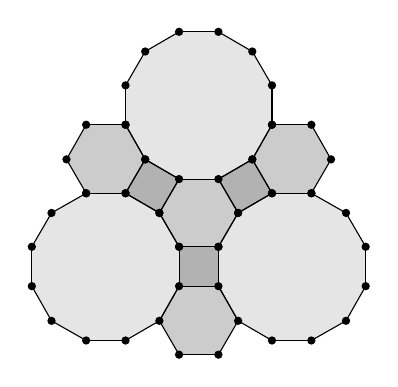
\begin{tikzpicture}[line cap=round,line join=round,>=triangle 45,x=1.0cm,y=1.0cm]
\fill[fill=black,fill opacity=0.2] (1.5,0) -- (2,0) -- (2.25,0.43) -- (2,0.87) -- (1.5,0.87) -- (1.25,0.43) -- cycle;
\fill[fill=black,fill opacity=0.1] (1.25,0.43) -- (1.5,0.87) -- (1.5,1.37) -- (1.25,1.8) -- (0.82,2.05) -- (0.32,2.05) -- (-0.12,1.8) -- (-0.37,1.37) -- (-0.37,0.87) -- (-0.12,0.43) -- (0.32,0.18) -- (0.82,0.18) -- cycle;
\fill[fill=black,fill opacity=0.1] (2,0.87) -- (2.25,0.43) -- (2.68,0.18) -- (3.18,0.18) -- (3.62,0.43) -- (3.87,0.87) -- (3.87,1.37) -- (3.62,1.8) -- (3.18,2.05) -- (2.68,2.05) -- (2.25,1.8) -- (2,1.37) -- cycle;
\fill[fill=black,fill opacity=0.3] (1.5,0.87) -- (2,0.87) -- (2,1.37) -- (1.5,1.37) -- cycle;
\fill[fill=black,fill opacity=0.2] (1.5,1.37) -- (2,1.37) -- (2.25,1.8) -- (2,2.23) -- (1.5,2.23) -- (1.25,1.8) -- cycle;
\fill[fill=black,fill opacity=0.1] (1.5,2.23) -- (2,2.23) -- (2.43,2.48) -- (2.68,2.92) -- (2.68,3.42) -- (2.43,3.85) -- (2,4.1) -- (1.5,4.1) -- (1.07,3.85) -- (0.82,3.42) -- (0.82,2.92) -- (1.07,2.48) -- cycle;
\fill[fill=black,fill opacity=0.3] (2,2.23) -- (2.25,1.8) -- (2.68,2.05) -- (2.43,2.48) -- cycle;
\fill[fill=black,fill opacity=0.3] (1.25,1.8) -- (1.5,2.23) -- (1.07,2.48) -- (0.82,2.05) -- cycle;
\fill[fill=black,fill opacity=0.2] (0.82,2.05) -- (1.07,2.48) -- (0.82,2.92) -- (0.32,2.92) -- (0.07,2.48) -- (0.32,2.05) -- cycle;
\fill[fill=black,fill opacity=0.2] (2.43,2.48) -- (2.68,2.05) -- (3.18,2.05) -- (3.43,2.48) -- (3.18,2.92) -- (2.68,2.92) -- cycle;
\draw (1.5,0)-- (2,0);
\draw (2,0)-- (2.25,0.43);
\draw (2.25,0.43)-- (2,0.87);
\draw (2,0.87)-- (1.5,0.87);
\draw (1.5,0.87)-- (1.25,0.43);
\draw (1.25,0.43)-- (1.5,0);
\draw (1.25,0.43)-- (1.5,0.87);
\draw (1.5,0.87)-- (1.5,1.37);
\draw (1.5,1.37)-- (1.25,1.8);
\draw (1.25,1.8)-- (0.82,2.05);
\draw (0.82,2.05)-- (0.32,2.05);
\draw (0.32,2.05)-- (-0.12,1.8);
\draw (-0.12,1.8)-- (-0.37,1.37);
\draw (-0.37,1.37)-- (-0.37,0.87);
\draw (-0.37,0.87)-- (-0.12,0.43);
\draw (-0.12,0.43)-- (0.32,0.18);
\draw (0.32,0.18)-- (0.82,0.18);
\draw (0.82,0.18)-- (1.25,0.43);
\draw (2,0.87)-- (2.25,0.43);
\draw (2.25,0.43)-- (2.68,0.18);
\draw (2.68,0.18)-- (3.18,0.18);
\draw (3.18,0.18)-- (3.62,0.43);
\draw (3.62,0.43)-- (3.87,0.87);
\draw (3.87,0.87)-- (3.87,1.37);
\draw (3.87,1.37)-- (3.62,1.8);
\draw (3.62,1.8)-- (3.18,2.05);
\draw (3.18,2.05)-- (2.68,2.05);
\draw (2.68,2.05)-- (2.25,1.8);
\draw (2.25,1.8)-- (2,1.37);
\draw (2,1.37)-- (2,0.87);
\draw (1.5,0.87)-- (2,0.87);
\draw (2,0.87)-- (2,1.37);
\draw (2,1.37)-- (1.5,1.37);
\draw (1.5,1.37)-- (1.5,0.87);
\draw (1.5,1.37)-- (2,1.37);
\draw (2,1.37)-- (2.25,1.8);
\draw (2.25,1.8)-- (2,2.23);
\draw (2,2.23)-- (1.5,2.23);
\draw (1.5,2.23)-- (1.25,1.8);
\draw (1.25,1.8)-- (1.5,1.37);
\draw (1.5,2.23)-- (2,2.23);
\draw (2,2.23)-- (2.43,2.48);
\draw (2.43,2.48)-- (2.68,2.92);
\draw (2.68,2.92)-- (2.68,3.42);
\draw (2.68,3.42)-- (2.43,3.85);
\draw (2.43,3.85)-- (2,4.1);
\draw (2,4.1)-- (1.5,4.1);
\draw (1.5,4.1)-- (1.07,3.85);
\draw (1.07,3.85)-- (0.82,3.42);
\draw (0.82,3.42)-- (0.82,2.92);
\draw (0.82,2.92)-- (1.07,2.48);
\draw (1.07,2.48)-- (1.5,2.23);
\draw (2,2.23)-- (2.25,1.8);
\draw (2.25,1.8)-- (2.68,2.05);
\draw (2.68,2.05)-- (2.43,2.48);
\draw (2.43,2.48)-- (2,2.23);
\draw (1.25,1.8)-- (1.5,2.23);
\draw (1.5,2.23)-- (1.07,2.48);
\draw (1.07,2.48)-- (0.82,2.05);
\draw (0.82,2.05)-- (1.25,1.8);
\draw (0.82,2.05)-- (1.07,2.48);
\draw (1.07,2.48)-- (0.82,2.92);
\draw (0.82,2.92)-- (0.32,2.92);
\draw (0.32,2.92)-- (0.07,2.48);
\draw (0.07,2.48)-- (0.32,2.05);
\draw (0.32,2.05)-- (0.82,2.05);
\draw (2.43,2.48)-- (2.68,2.05);
\draw (2.68,2.05)-- (3.18,2.05);
\draw (3.18,2.05)-- (3.43,2.48);
\draw (3.43,2.48)-- (3.18,2.92);
\draw (3.18,2.92)-- (2.68,2.92);
\draw (2.68,2.92)-- (2.43,2.48);
\begin{scriptsize}
\fill [color=black] (1.5,0) circle (1.5pt);
\fill [color=black] (2,0) circle (1.5pt);
\fill [color=black] (2.25,0.43) circle (1.5pt);
\fill [color=black] (2,0.87) circle (1.5pt);
\fill [color=black] (1.5,0.87) circle (1.5pt);
\fill [color=black] (1.25,0.43) circle (1.5pt);
\fill [color=black] (1.5,1.37) circle (1.5pt);
\fill [color=black] (1.25,1.8) circle (1.5pt);
\fill [color=black] (0.82,2.05) circle (1.5pt);
\fill [color=black] (0.32,2.05) circle (1.5pt);
\fill [color=black] (-0.12,1.8) circle (1.5pt);
\fill [color=black] (-0.37,1.37) circle (1.5pt);
\fill [color=black] (-0.37,0.87) circle (1.5pt);
\fill [color=black] (-0.12,0.43) circle (1.5pt);
\fill [color=black] (0.32,0.18) circle (1.5pt);
\fill [color=black] (0.82,0.18) circle (1.5pt);
\fill [color=black] (2.68,0.18) circle (1.5pt);
\fill [color=black] (3.18,0.18) circle (1.5pt);
\fill [color=black] (3.62,0.43) circle (1.5pt);
\fill [color=black] (3.87,0.87) circle (1.5pt);
\fill [color=black] (3.87,1.37) circle (1.5pt);
\fill [color=black] (3.62,1.8) circle (1.5pt);
\fill [color=black] (3.18,2.05) circle (1.5pt);
\fill [color=black] (2.68,2.05) circle (1.5pt);
\fill [color=black] (2.25,1.8) circle (1.5pt);
\fill [color=black] (2,1.37) circle (1.5pt);
\fill [color=black] (2,1.37) circle (1.5pt);
\fill [color=black] (1.5,1.37) circle (1.5pt);
\fill [color=black] (2.25,1.8) circle (1.5pt);
\fill [color=black] (2,2.23) circle (1.5pt);
\fill [color=black] (1.5,2.23) circle (1.5pt);
\fill [color=black] (1.25,1.8) circle (1.5pt);
\fill [color=black] (2.43,2.48) circle (1.5pt);
\fill [color=black] (2.68,2.92) circle (1.5pt);
\fill [color=black] (2.68,3.42) circle (1.5pt);
\fill [color=black] (2.43,3.85) circle (1.5pt);
\fill [color=black] (2,4.1) circle (1.5pt);
\fill [color=black] (1.5,4.1) circle (1.5pt);
\fill [color=black] (1.07,3.85) circle (1.5pt);
\fill [color=black] (0.82,3.42) circle (1.5pt);
\fill [color=black] (0.82,2.92) circle (1.5pt);
\fill [color=black] (1.07,2.48) circle (1.5pt);
\fill [color=black] (2.68,2.05) circle (1.5pt);
\fill [color=black] (2.43,2.48) circle (1.5pt);
\fill [color=black] (1.07,2.48) circle (1.5pt);
\fill [color=black] (0.82,2.05) circle (1.5pt);
\fill [color=black] (0.82,2.92) circle (1.5pt);
\fill [color=black] (0.32,2.92) circle (1.5pt);
\fill [color=black] (0.07,2.48) circle (1.5pt);
\fill [color=black] (0.32,2.05) circle (1.5pt);
\fill [color=black] (3.18,2.05) circle (1.5pt);
\fill [color=black] (3.43,2.48) circle (1.5pt);
\fill [color=black] (3.18,2.92) circle (1.5pt);
\fill [color=black] (2.68,2.92) circle (1.5pt);
\end{scriptsize}
\end{tikzpicture}
\end{center}
b) A tizenkétszög felbontható háromszögekre,
négyszögekre és hatszögekre a következő módon:
\begin{center}
    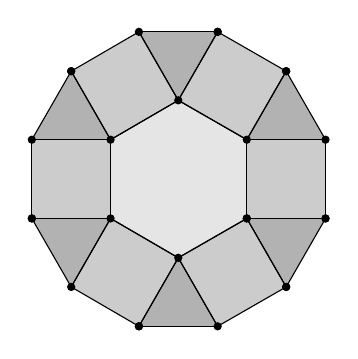
\begin{tikzpicture}[line cap=round,line join=round,>=triangle 45,x=1.0cm,y=1.0cm]
\fill[fill=black,fill opacity=0.1] (3,1) -- (3,2) -- (2.13,2.5) -- (1.27,2) -- (1.27,1) -- (2.13,0.5) -- cycle;
\fill[fill=black,fill opacity=0.2] (4,2) -- (3,2) -- (3,1) -- (4,1) -- cycle;
\fill[fill=black,fill opacity=0.3] (4,1) -- (3,1) -- (3.5,0.13) -- cycle;
\fill[fill=black,fill opacity=0.2] (3,1) -- (2.13,0.5) -- (2.63,-0.37) -- (3.5,0.13) -- cycle;
\fill[fill=black,fill opacity=0.2] (2.13,0.5) -- (1.27,1) -- (0.77,0.13) -- (1.63,-0.37) -- cycle;
\fill[fill=black,fill opacity=0.2] (1.27,1) -- (1.27,2) -- (0.27,2) -- (0.27,1) -- cycle;
\fill[fill=black,fill opacity=0.2] (1.27,2) -- (2.13,2.5) -- (1.63,3.37) -- (0.77,2.87) -- cycle;
\fill[fill=black,fill opacity=0.2] (2.13,2.5) -- (3,2) -- (3.5,2.87) -- (2.63,3.37) -- cycle;
\fill[fill=black,fill opacity=0.3] (3,2) -- (4,2) -- (3.5,2.87) -- cycle;
\fill[fill=black,fill opacity=0.3] (2.63,-0.37) -- (2.13,0.5) -- (1.63,-0.37) -- cycle;
\fill[fill=black,fill opacity=0.3] (0.77,0.13) -- (1.27,1) -- (0.27,1) -- cycle;
\fill[fill=black,fill opacity=0.3] (0.27,2) -- (1.27,2) -- (0.77,2.87) -- cycle;
\fill[fill=black,fill opacity=0.3] (1.63,3.37) -- (2.13,2.5) -- (2.63,3.37) -- cycle;
\draw (3,1)-- (3,2);
\draw (3,2)-- (2.13,2.5);
\draw (2.13,2.5)-- (1.27,2);
\draw (1.27,2)-- (1.27,1);
\draw (1.27,1)-- (2.13,0.5);
\draw (2.13,0.5)-- (3,1);
\draw (4,2)-- (3,2);
\draw (3,2)-- (3,1);
\draw (3,1)-- (4,1);
\draw (4,1)-- (4,2);
\draw (4,1)-- (3,1);
\draw (3,1)-- (3.5,0.13);
\draw (3.5,0.13)-- (4,1);
\draw (3,1)-- (2.13,0.5);
\draw (2.13,0.5)-- (2.63,-0.37);
\draw (2.63,-0.37)-- (3.5,0.13);
\draw (3.5,0.13)-- (3,1);
\draw (2.13,0.5)-- (1.27,1);
\draw (1.27,1)-- (0.77,0.13);
\draw (0.77,0.13)-- (1.63,-0.37);
\draw (1.63,-0.37)-- (2.13,0.5);
\draw (1.27,1)-- (1.27,2);
\draw (1.27,2)-- (0.27,2);
\draw (0.27,2)-- (0.27,1);
\draw (0.27,1)-- (1.27,1);
\draw (1.27,2)-- (2.13,2.5);
\draw (2.13,2.5)-- (1.63,3.37);
\draw (1.63,3.37)-- (0.77,2.87);
\draw (0.77,2.87)-- (1.27,2);
\draw (2.13,2.5)-- (3,2);
\draw (3,2)-- (3.5,2.87);
\draw (3.5,2.87)-- (2.63,3.37);
\draw (2.63,3.37)-- (2.13,2.5);
\draw (3,2)-- (4,2);
\draw (4,2)-- (3.5,2.87);
\draw (3.5,2.87)-- (3,2);
\draw (2.63,-0.37)-- (2.13,0.5);
\draw (2.13,0.5)-- (1.63,-0.37);
\draw (1.63,-0.37)-- (2.63,-0.37);
\draw (0.77,0.13)-- (1.27,1);
\draw (1.27,1)-- (0.27,1);
\draw (0.27,1)-- (0.77,0.13);
\draw (0.27,2)-- (1.27,2);
\draw (1.27,2)-- (0.77,2.87);
\draw (0.77,2.87)-- (0.27,2);
\draw (1.63,3.37)-- (2.13,2.5);
\draw (2.13,2.5)-- (2.63,3.37);
\draw (2.63,3.37)-- (1.63,3.37);
\begin{scriptsize}
\fill [color=black] (3,1) circle (1.5pt);
\fill [color=black] (3,2) circle (1.5pt);
\fill [color=black] (2.13,2.5) circle (1.5pt);
\fill [color=black] (1.27,2) circle (1.5pt);
\fill [color=black] (1.27,1) circle (1.5pt);
\fill [color=black] (2.13,0.5) circle (1.5pt);
\fill [color=black] (4,2) circle (1.5pt);
\fill [color=black] (4,1) circle (1.5pt);
\fill [color=black] (3,1) circle (1.5pt);
\fill [color=black] (4,1) circle (1.5pt);
\fill [color=black] (3.5,0.13) circle (1.5pt);
\fill [color=black] (2.63,-0.37) circle (1.5pt);
\fill [color=black] (3.5,0.13) circle (1.5pt);
\fill [color=black] (0.77,0.13) circle (1.5pt);
\fill [color=black] (1.63,-0.37) circle (1.5pt);
\fill [color=black] (0.27,2) circle (1.5pt);
\fill [color=black] (0.27,1) circle (1.5pt);
\fill [color=black] (1.63,3.37) circle (1.5pt);
\fill [color=black] (0.77,2.87) circle (1.5pt);
\fill [color=black] (3.5,2.87) circle (1.5pt);
\fill [color=black] (2.63,3.37) circle (1.5pt);
\fill [color=black] (3.5,2.87) circle (1.5pt);
\fill [color=black] (1.63,-0.37) circle (1.5pt);
\fill [color=black] (0.27,1) circle (1.5pt);
\fill [color=black] (0.77,2.87) circle (1.5pt);
\fill [color=black] (2.63,3.37) circle (1.5pt);
\end{scriptsize}
\end{tikzpicture}
\end{center}
A megoldáshoz a továbbiakban használjuk a 11. osztály
hatodik feladatának a meg\-ol\-dá\-sá\-hoz készített
utolsó ábrát: a koordináta-rendszert, amelyben egy
tizenkétszög középpontja az origó és  két szomszédos
vízszintes tizenkétszög középpontja között a
távolság egy egység.

Megadunk egy lehetséges szerkesztést. Az összes olyan
ti\-zen\-két\-szög\-re, amelyek középpontjának a
koordinátái nem $(2^k,2^k)$ ala\-kúak ($k\in \mathbb{N}$,
$k\ge 1$) használjuk az előző felbontást. Az így
keletkezett síklefödés esetén végtelen sok olyan
mintázat létezik, amelyik véges sokszor fordul csak elő: az
összes olyan mintázat, amelyik pontosan két megmaradt,
egymást követő ti\-zen\-két\-szöget és a köztük
levő szabályos sokszögek által kitöltött alakzatot
tartalmazza, csak egyszer fordul elő. Valóban, a
szerkesztésünk kö\-vet\-kez\-mé\-nye, hogy két ilyen
tizenkétszög középpontjának a távolsága egyre
na\-gyobb.




\end{document}